\begin{frame}[fragile] 
%--------------------------------------------------
\frametitle{\cello\ Mesh data structure}
\framesubtitle{AMR design philosophy}
%--------------------------------------------------
%  AMR:        additional level of refinement: patches + blocks
%  AMR:        new [currently proprietary] enhancement for "large, shallow" AMR
%  AMR:        new [currently proprietary] enhancement for "deep, targeted" AMR
%  AMR:        no level jumps, symmetric refinement for symmetric problems
%  AMR:        ghost zones optionally allocated only when needed
\begin{itemize}
\small
\item Decouple mesh refinement from data distribution
  \begin{itemize}
  \item in Enzo,   \code{grid} $=$ parallel task 
  \item in Cello,  \code{Patch} $\supseteq$ \code{Block} $=$ parallel task
  \item \code{Block} size can be optimized independently of \code{Patch} size
       \begin{itemize}
       \item target specialized computational kernels
       \item increased parallelism
       \item improved load balancing
       \item reduced memory fragmentation
       \end{itemize}
  \end{itemize}
\item ``Unigrid'' when possible; AMR when necessary
  \begin{itemize}
  \item leverage unigrid performance and scalability
  \item \code{Patch}es encapsulate parallel unigrid subproblems
  \item $O(1)$ metadata for full unigrid problem ($O(P)$ for Enzo)
  \end{itemize}
\end{itemize}

\end{frame}

\begin{frame}[fragile] 
%--------------------------------------------------
\frametitle{\cello\ Mesh data structure}
\framesubtitle{Core \code{Mesh} classes}
%--------------------------------------------------
%  AMR:        additional level of refinement: patches + blocks
%  AMR:        new [currently proprietary] enhancement for "large, shallow" AMR
%  AMR:        new [currently proprietary] enhancement for "deep, targeted" AMR
%  AMR:        no level jumps, symmetric refinement for symmetric problems
%  AMR:        ghost zones optionally allocated only when needed
\begin{center}
\begin{minipage}{2.2in}
\centerline{ Mesh} \ \\
\centerline{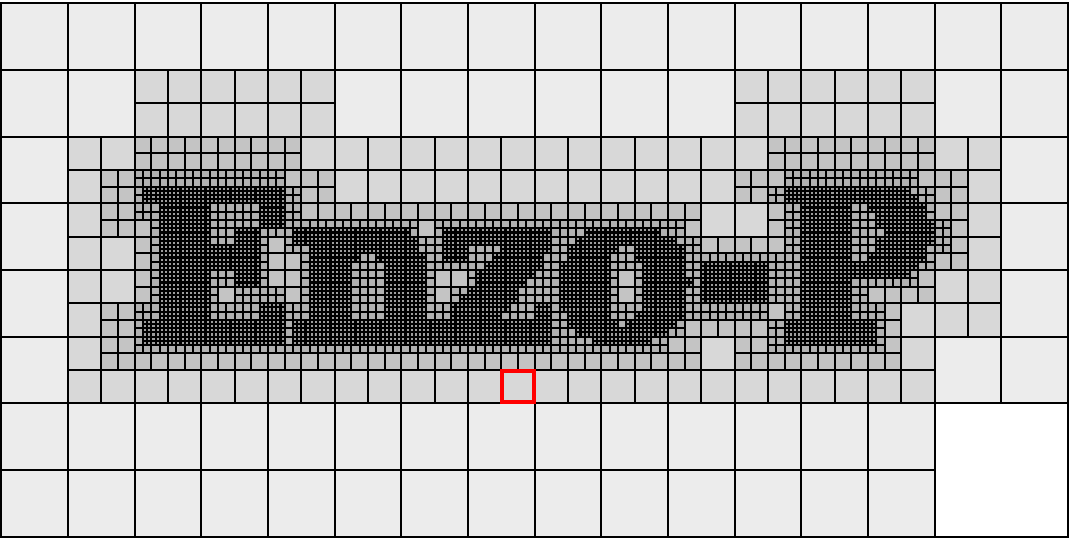
\includegraphics[width=2in]{amr-hierarchy.pdf}}
\end{minipage} \ \\ \vspace{0.1in}
\begin{minipage}{2.2in}
\centerline{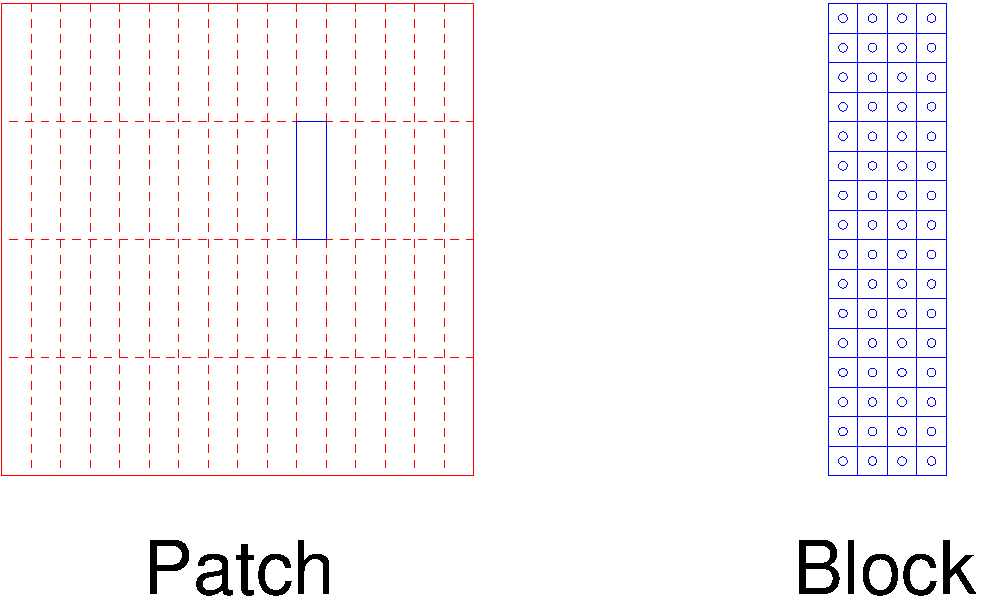
\includegraphics[width=1.6in]{amr-patch.pdf}}
\end{minipage} \ \\
\end{center}
\end{frame}

\begin{frame}[fragile] 
%--------------------------------------------------
\frametitle{\cello\ Mesh data structure}
\framesubtitle{\code{Mesh} related classes}
%--------------------------------------------------
%  AMR:        additional level of refinement: patches + blocks
%  AMR:        new [currently proprietary] enhancement for "large, shallow" AMR
%  AMR:        new [currently proprietary] enhancement for "deep, targeted" AMR
%  AMR:        no level jumps, symmetric refinement for symmetric problems
%  AMR:        ghost zones optionally allocated only when needed
\centerline{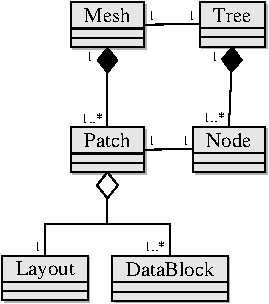
\includegraphics[width=2.5in]{uml/amr.pdf}}

\end{frame}

\begin{frame}[fragile] 
%--------------------------------------------------
\frametitle{\cello\ Mesh data structure}
\framesubtitle{\code{Mesh} related classes}
%--------------------------------------------------
%  AMR:        additional level of refinement: patches + blocks
%  AMR:        new [currently proprietary] enhancement for "large, shallow" AMR
%  AMR:        new [currently proprietary] enhancement for "deep, targeted" AMR
%  AMR:        no level jumps, symmetric refinement for symmetric problems
%  AMR:        ghost zones optionally allocated only when needed
\begin{itemize}
\small
\item \code{Mesh}: full AMR hierarchy
\item \code{Patch}: region of uniform resolution
  \begin{itemize}
  \item Cello unigrid problem degenerates to single \code{Patch}
  \end{itemize}
\item \code{Block}: basic distributed data unit / parallel task
  \begin{itemize}
  \item MPI: e.g.~one \code{Block} per process in Cartesian topology
  \item CHARM++: one \code{Block} per 3D ``chare array''
  \item GPU / OMP / UPC support planned
  \end{itemize}
\item \code{Layout}: specifies how to distribute \code{Block}s in a \code{Patch}
  \begin{itemize}
  \item \code{Block} size, process range, neighbor pointers, etc.
  \item hierarchical parallelism through multiple \code{Layout}s
  \end{itemize}
\item \code{Block} data: \code{Field}, \code{Particles}, etc.
\item \code{Tree}, \code{Node}: bare-bones octree data structure
  \begin{itemize}
  \item \code{Node}s are only objects replicated across machine
    \begin{itemize}
    \item small nodes: $\le 24$ bytes ($>1500$ bytes/\code{grid} for Enzo)
    \item fewer nodes: e.g.~$1$ instead of $P$ for unigrid case
    \end{itemize}
  \end{itemize}
\end{itemize}

\end{frame}





